\chapter[Metodologia]{Metodologia}
\label{cap:metodologia}

Este capítulo descreve o corpus, o pipeline de processamento, a estratégia de
particionamento, a geração de pares candidatos e o protocolo de avaliação. Todas
as etapas foram projetadas sob a premissa de \textbf{reprodutibilidade}: ordenação
determinística das saídas, serialização fixa, semente aleatória registrada e
verificação por \foreignlanguage{english}{hashes} SHA-256.

\section{Visão geral do pipeline}
\label{sec:pipeline}

Entende-se por \emph{pipeline} de PLN uma sequência encadeada de etapas em que a
saída de cada estágio é a entrada do seguinte, de modo que o dado bruto é
progressivamente transformado até a métrica final. Estruturar o trabalho como um
\emph{pipeline} explícito tem duas vantagens: isola a responsabilidade de cada
etapa (facilitando o teste e a auditoria isolados) e torna o caminho completo
\textbf{reproduzível}, pois cada estágio é determinístico e seus artefatos podem
ser verificados de forma independente. As etapas deste trabalho, na ordem em que
são executadas, são:

\begin{enumerate}
  \item \textbf{\emph{Parsing} (XML bruto $\rightarrow$ \texttt{dataset.jsonl}).}
        O \emph{parser} converte cada documento XML do SemClinBr em um registro
        canônico JSONL (texto, entidades e relações). É necessário porque o
        formato XML original, fiel à anotação, não é prático para as etapas
        seguintes; a representação canônica unifica o acesso ao corpus.
  \item \textbf{Particionamento (\texttt{dataset.jsonl} $\rightarrow$
        \emph{splits}).} O conjunto é dividido em treino, desenvolvimento e teste
        em nível de documento. É necessário para separar dados de ajuste dos de
        avaliação sem vazamento (Seção~\ref{sec:particao}).
  \item \textbf{Geração de pares candidatos (\emph{splits} $\rightarrow$
        candidatos rotulados).} Como o corpus só anota relações positivas, esta
        etapa constrói os exemplos negativos (\texttt{no\_relation}), produzindo o
        espaço de classificação completo (Seção~\ref{sec:candidatos}).
  \item \textbf{Marcação de entidades (candidatos $\rightarrow$ texto marcado).}
        Para os modelos contextuais, cada par candidato é transformado na string
        de entrada do \emph{encoder}, com marcadores de entidade tipados
        (Seção~\ref{sec:markers} do Capítulo~\ref{cap:prototipo}). É necessária
        para informar ao modelo \emph{quais} entidades formam o par e \emph{de que
        tipo} elas são.
  \item \textbf{Classificação (texto marcado $\rightarrow$ predições).} Cada
        \emph{baseline} ou modelo atribui um rótulo do conjunto
        \{\texttt{negation\_of}, \texttt{associated\_with}, \texttt{no\_relation}\}
        a cada candidato (Capítulo~\ref{cap:prototipo}).
  \item \textbf{Avaliação (predições $\rightarrow$ métricas).} As predições são
        comparadas ao \emph{gold} para produzir macro-F1, F1 por classe e
        intervalos de confiança, com testes pareados entre modelos
        (Seção~\ref{sec:avaliacao}).
\end{enumerate}

O \textbf{determinismo} é garantido em \emph{todas} as etapas, condição para que os
\emph{hashes} SHA-256 dos artefatos sejam estáveis entre execuções: a serialização
JSONL é fixada byte a byte (\texttt{ensure\_ascii=False}, \texttt{sort\_keys=True},
quebras de linha LF); a ordenação das saídas é explícita (documentos por
\texttt{doc\_id}, candidatos por $(\text{start},\text{end},\text{id})$); a semente
aleatória é fixada em $42$ e registrada em cada artefato de resultado; e o ambiente
de execução tem versões de bibliotecas pinadas. As seções seguintes detalham cada
etapa. A Figura~\ref{fig:semclinbr} (Seção~\ref{sec:corpus}) situa a origem do
dado de entrada, ilustrando o processo de criação e anotação do SemClinBr que
antecede o \emph{pipeline} aqui descrito.

\section{Corpus SemClinBr}
\label{sec:corpus}

O trabalho utiliza o corpus SemClinBr \cite{oliveira_2022_semclinbr}, composto por
mil documentos clínicos em português anotados com entidades e relações. O corpus
é distribuído sob licença restrita, mediante solicitação formal, e seus arquivos
XML originais são tratados como \textbf{imutáveis} ao longo do pipeline. As
relações anotadas no corpus público utilizado pertencem a dois tipos,
\texttt{associated\_with} e \texttt{negation\_of}, sobre os quais se constrói o
espaço de rótulos da tarefa. A Figura~\ref{fig:semclinbr} ilustra o processo de
criação e anotação do corpus.

\begin{figure}[H]
    \centering
    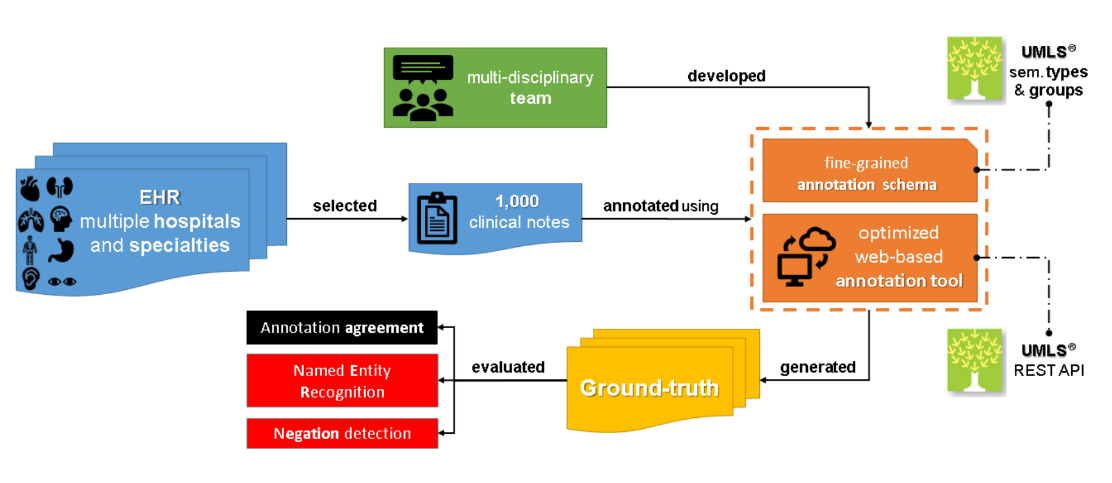
\includegraphics[width=0.90\textwidth]{imagens/processo-semclinbr.png}
    \caption{ Processo de criação e anotação do corpus SemClinBr }
    \label{fig:semclinbr}

    {\footnotesize Fonte: Oliveira et al. (2022).}
\end{figure}

\section{Parsing e representação canônica}

Um parser converte cada arquivo XML em um registro canônico no formato JSONL, com
identificador do documento, texto, lista de entidades (tipo e \emph{offsets}) e
lista de relações. O parser é \emph{fiel ao XML}: não normaliza tipos de entidade
ou de relação, deixando tais decisões para etapas posteriores. A única
transformação aplicada ao texto é o colapso de quebras de linha
(\texttt{\textbackslash r\textbackslash n}, \texttt{\textbackslash r},
\texttt{\textbackslash n}) em espaço único, necessário para manter o alinhamento
dos \emph{offsets} de anotação.

Por se tratar de um corpus com inconsistências de anotação conhecidas, o parser
executa verificações de sanidade (correspondência entre o texto extraído por
\emph{offset} e o atributo anotado, validade dos intervalos e integridade
referencial das relações) e, quando possível, corrige automaticamente pequenos
deslocamentos de \emph{offset} ($\pm 1$ e $\pm 2$ caracteres). As inconsistências
são acumuladas em um log de avisos em vez de interromperem o processamento.

\section{Caracterização do corpus}

A análise exploratória (\foreignlanguage{english}{Exploratory Data Analysis}, EDA)
foi conduzida sobre a representação canônica do corpus, totalizando $1\,000$
documentos, $45\,132$ entidades (média de $45{,}1$ por documento) e $11\,353$
relações (média de $11{,}4$ por documento). A mediana é de $10$ relações por
documento, o percentil 90 é de $24$ e o máximo observado é de $63$; $46$
documentos ($4{,}60\%$) não possuem nenhuma relação anotada. Essa caracterização
quantifica a distribuição das relações, a distância entre entidades relacionadas e
as categorias de entidade, fornecendo subsídio empírico para as decisões de
projeto das etapas seguintes.

\subsection{Distribuição dos tipos de relação}

A Tabela~\ref{tab:distribuicao} e a \autoref{fig:eda_reltype} mostram o forte
desbalanceamento entre os dois tipos de relação anotados, com predominância de
\texttt{associated\_with} ($86{,}07\%$) sobre \texttt{negation\_of} ($13{,}93\%$).
Esse desequilíbrio motiva tanto a escolha do macro-F1 como métrica principal
quanto o tratamento explícito de classes nos modelos aprendidos.

\begin{table}[htbp]
  \centering
  \caption{Distribuição dos tipos de relação no corpus parseado.}
  \label{tab:distribuicao}
  % gerado por scripts/eda/eda_relations.py — NÃO EDITAR À MÃO
% (cópia de paper/tables/eda_reltype_distribution.tex)
\begin{tabular}{lrr}
\toprule
Tipo de relação & N & \% \\
\midrule
\texttt{associated\_with} & 9772 & 86.07 \\
\texttt{negation\_of} & 1581 & 13.93 \\
\midrule
\textbf{Total} & \textbf{11353} & 100.00 \\
\bottomrule
\end{tabular}
\\[4pt]
  {\footnotesize Fonte: elaborado pelo autor a partir do SemClinBr.}
\end{table}

\begin{figure}[htbp]
  \centering
  \caption{Distribuição dos tipos de relação no SemClinBr.}
  \label{fig:eda_reltype}
  
\includegraphics[width=0.6\textwidth]{eda/01_reltype_distribution.png}\\[4pt]
  {\footnotesize Fonte: elaborado pelo autor (\texttt{scripts/eda/eda\_relations.py}).}
\end{figure}

\subsection{Distância entre entidades relacionadas}

A Tabela~\ref{tab:distancia} e a \autoref{fig:eda_dist}
indicam que as relações ocorrem entre entidades próximas: a mediana da distância é
de poucos caracteres e o percentil 95 não ultrapassa algumas dezenas
(\texttt{associated\_with}: média $11{,}9$, p95 $43$; \texttt{negation\_of}: média
$3{,}5$, p95 $15$). Essa observação fundamenta diretamente a escolha da janela
máxima (\texttt{max\_gap}$=200$) na geração de pares candidatos.

\begin{table}[htbp]
  \centering
  \caption{Estatísticas da distância (em caracteres) entre entidades relacionadas, por tipo.}
  \label{tab:distancia}
  \resizebox{\textwidth}{!}{% gerado por scripts/eda/eda_relations.py — NÃO EDITAR À MÃO
% (cópia de paper/tables/eda_distance_by_type.tex)
\begin{tabular}{lrrrrrrr}
\toprule
Tipo & N & média & p25 & p50 & p75 & p90 & p95 \\
\midrule
\texttt{associated\_with} & 9772 & 11.9 & 1 & 4 & 10 & 25 & 43 \\
\texttt{negation\_of} & 1581 & 3.5 & 1 & 1 & 1 & 11 & 15 \\
\bottomrule
\end{tabular}
}\\[4pt]
  {\footnotesize Fonte: elaborado pelo autor a partir do SemClinBr.}
\end{table}

\begin{figure}[htbp]
  \centering
  \caption{Distribuição da distância em caracteres entre entidades relacionadas (recorte em 200).}
  \label{fig:eda_dist}
  
\includegraphics[width=0.7\textwidth]{eda/02_distance_all_clip200.png}\\[4pt]
  {\footnotesize Fonte: elaborado pelo autor (\texttt{scripts/eda/eda\_relations.py}).}
\end{figure}

\subsection{Relações por documento e categorias de entidade}

A \autoref{fig:eda_relsdoc} apresenta a distribuição do número de relações por
documento, e a \autoref{fig:eda_entcat}, as categorias de entidade mais frequentes
(após decomposição das anotações multirrótulo separadas por ``|''). As categorias
predominantes --- \texttt{Abbreviation} ($12\,502$), \texttt{Finding} ($6\,806$),
\texttt{Therapeutic or Preventive Procedure} ($4\,737$) e \texttt{Sign or Symptom}
($4\,579$) --- refletem a natureza telegráfica e abreviada do texto clínico. Vale
notar a presença expressiva da categoria \texttt{Negation} ($2\,616$), coerente
com a importância do fenômeno de negação tratado neste trabalho.

\begin{figure}[htbp]
  \centering
  \caption{Distribuição do número de relações por documento.}
  \label{fig:eda_relsdoc}
  
\includegraphics[width=0.7\textwidth]{eda/03_relations_per_doc.png}\\[4pt]
  {\footnotesize Fonte: elaborado pelo autor (\texttt{scripts/eda/eda\_relations.py}).}
\end{figure}

\begin{figure}[htbp]
  \centering
  \caption{Categorias atômicas de entidade mais frequentes (top 25).}
  \label{fig:eda_entcat}
  
\includegraphics[width=0.9\textwidth]{eda/04_entity_categories_atomic.png}\\[4pt]
  {\footnotesize Fonte: elaborado pelo autor (\texttt{scripts/eda/eda\_relations.py}).}
\end{figure}

\section{Particionamento dos dados}
\label{sec:particao}

A partição segue a razão 80/10/10 em \textbf{nível de documento}, e não de
relação. Essa escolha previne o vazamento de dados: relações de um mesmo documento
compartilham vocabulário e trechos repetidos, e dividi-las entre partições
diferentes inflaria artificialmente as métricas de teste. A partição é
\textbf{estratificada} pela presença das classes \texttt{negation\_of} e
\texttt{associated\_with} em cada documento, por meio do algoritmo de
estratificação multirrótulo de \citeonline{sechidis_2011_stratification}, de modo
a garantir representação estável da classe minoritária em todas as partições.

A partição é gerada com semente fixa ($42$) e \textbf{congelada}: os arquivos de
treino, desenvolvimento e teste e seus respectivos \emph{hashes} SHA-256 são
versionados (Apêndice~\ref{ap:sha256}), evitando que comparações entre execuções
sejam confundidas com variação de amostragem. O resultado são $800$ documentos de
treino, $100$ de desenvolvimento e $100$ de teste.

A Tabela~\ref{tab:particao} apresenta a distribuição real das relações entre as
partições. O ponto crítico é que a classe minoritária \texttt{negation\_of}, que
representa apenas $13{,}93\%$ das relações do corpus, mantém proporção estável em
todas as partições (entre $13{,}74\%$ e $14{,}96\%$). Essa preservação confirma o
funcionamento do algoritmo de estratificação multirrótulo de
\citeonline{sechidis_2011_stratification}: um particionamento puramente aleatório
poderia, por azar de amostragem, sub-representar \texttt{negation\_of} no conjunto
de teste, comprometendo a estabilidade da estimativa de F1 dessa classe. A
estratificação por presença simultânea das duas classes evita esse risco e torna
as métricas por classe comparáveis entre as partições.

\begin{table}[htbp]
  \centering
  \caption{Distribuição real das relações por partição (\emph{splits} congelados, semente 42).}
  \label{tab:particao}
  \resizebox{\textwidth}{!}{%
  \begin{tabular}{lrrrrr}
  \toprule
  Partição & Documentos & \texttt{associated\_with} & \texttt{negation\_of} & Total relações & \% \texttt{negation\_of} \\
  \midrule
  Treino & 800  & 7854 & 1251 & 9105  & 13,74 \\
  Dev    & 100  & 955  & 168  & 1123  & 14,96 \\
  Teste  & 100  & 963  & 162  & 1125  & 14,40 \\
  \midrule
  \textbf{Total} & \textbf{1000} & \textbf{9772} & \textbf{1581} & \textbf{11353} & \textbf{13,93} \\
  \bottomrule
  \end{tabular}}\\[4pt]
  {\footnotesize Fonte: elaborado pelo autor (\texttt{data/splits/split\_stats.json}).}
\end{table}

A \autoref{fig:split_dist} apresenta a mesma informação em barras agrupadas (escala
logarítmica), evidenciando visualmente que a proporção da classe minoritária
\texttt{negation\_of} permanece estável ($13{,}7\%$, $15{,}0\%$ e $14{,}4\%$ em
treino, desenvolvimento e teste). A constância dessa proporção, apesar de a
partição ser feita por documento e não por relação, é exatamente o efeito da
estratificação multirrótulo: a classe rara não é sub-representada em nenhuma
partição, condição necessária para que a estimativa de F1 de \texttt{negation\_of}
no teste seja confiável.

\begin{figure}[htbp]
  \centering
  \caption{Distribuição das relações por partição (escala logarítmica), com o percentual de \texttt{negation\_of} anotado.}
  \label{fig:split_dist}
  
\includegraphics[width=0.75\textwidth]{eda/05_relations_by_split.png}\\[4pt]
  {\footnotesize Fonte: elaborado pelo autor (\texttt{scripts/eda/plot\_split\_distribution.py}).}
\end{figure}

\section{Geração de pares candidatos}
\label{sec:candidatos}

O SemClinBr anota apenas relações \emph{positivas}: cada relação registrada indica
que existe vínculo entre duas entidades, mas a ausência de anotação não é, por si,
um exemplo negativo explícito. Avaliar um classificador no espaço
\{\texttt{negation\_of}, \texttt{associated\_with}, \texttt{no\_relation}\} exige,
portanto, \textbf{construir} os exemplos negativos. Treinar ou avaliar apenas com
os pares anotados produziria um classificador binário sobre as duas classes
positivas, incapaz de operar em um cenário real, em que o sistema recebe \emph{todos}
os pares de entidades de um documento e precisa decidir, para cada um, se há relação
e de que tipo. A classe \texttt{no\_relation} é o que torna a tarefa aplicável fora
do conjunto anotado.

A geração é feita pela função \texttt{iter\_candidate\_pairs}
(\texttt{scripts/utils/candidates.py}), compartilhada por todos os modelos e
\emph{baselines} --- condição necessária para que os resultados fiquem na mesma
régua estatística. Para cada documento, ela percorre todos os \textbf{pares
ordenados} de entidades $(e_1, e_2)$, $e_1 \neq e_2$ --- a ordem importa porque a
direção é relevante para a negação ---, descarta os pares cuja distância em
caracteres exceda a janela máxima (\texttt{max\_gap}$=200$) e os pares entre
documentos distintos, e atribui o rótulo: se o par ordenado $(e_1, e_2)$ coincide
com uma relação anotada, recebe o tipo \emph{gold}; caso contrário, recebe
\texttt{no\_relation}. A emissão segue ordenação determinística por
$(\text{start}, \text{end}, \text{id})$, de modo que o conjunto de candidatos --- e
o \emph{hash} das predições --- seja estável entre execuções.

Em resumo, o gerador respeita cinco propriedades, todas verificadas por testes
automatizados (\texttt{tests/test\_determinism.py}): \textbf{(i) ordenação
determinística} --- os pares são emitidos sempre na mesma ordem por
$(\text{start}, \text{end}, \text{id})$ de $e_1$ e depois de $e_2$, requisito do
qual depende o \emph{hash} SHA-256 das predições; \textbf{(ii) sem cruzamento entre
documentos} --- nunca se forma um par com entidades de documentos distintos, pois o
documento é a unidade de processamento; \textbf{(iii) janela respeitada} --- apenas
pares cuja distância em caracteres (entre o fim de $e_1$ e o início de $e_2$) seja
$\leq \texttt{max\_gap}=200$ são gerados; \textbf{(iv) sem autopares} --- nunca se
forma o par $(e, e)$ de uma entidade consigo mesma ($e_1 \neq e_2$); e \textbf{(v)
conferência com o \emph{gold}} --- um par presente nas relações anotadas do
documento recebe o tipo real (\texttt{associated\_with} ou \texttt{negation\_of}),
e um par ausente recebe \texttt{no\_relation} (amostragem negativa).

A \autoref{quad:exemplo_candidatos} ilustra o processo em um trecho real do corpus.
A relação anotada é $16 \rightarrow 52 = \texttt{negation\_of}$ (a entidade
``NÃO ESPECIFICADA'' nega ``OSTEOMIELITE''). Das seis combinações ordenadas
possíveis entre as três entidades próximas, apenas o par $(16, 52)$ casa com o
\emph{gold}; os outros cinco tornam-se \texttt{no\_relation}. A representação de
entrada para os modelos contextuais marca o par com delimitadores tipados, por
exemplo \texttt{[E1] DISO : OSTEOMIELITE [/E1] [E2] Negation : NÃO ESPECIFICADA
[/E2]}.

\begin{quadro}[htbp]
  \centering
  \caption{Exemplo de geração de candidatos para um trecho do SemClinBr.}
  \label{quad:exemplo_candidatos}
  \resizebox{\textwidth}{!}{%
  \begin{tabular}{lll}
  \toprule
  \multicolumn{3}{l}{Entidades: \texttt{16}=``OSTEOMIELITE'' (\emph{Disease or Syndrome}),
  \texttt{52}=``NÃO ESPECIFICADA'' (\emph{Negation}),} \\
  \multicolumn{3}{l}{\texttt{17}=``INTUBADO'' (\emph{Finding}). Relação \emph{gold}:
  $16 \rightarrow 52 = \texttt{negation\_of}$.} \\
  \midrule
  Par ordenado & Rótulo gerado & \\
  \midrule
  $16 \rightarrow 52$ & \texttt{negation\_of}  & (casa com o \emph{gold}) \\
  $16 \rightarrow 17$ & \texttt{no\_relation}  & \\
  $52 \rightarrow 16$ & \texttt{no\_relation}  & (direção inversa do \emph{gold}) \\
  $52 \rightarrow 17$ & \texttt{no\_relation}  & \\
  $17 \rightarrow 16$ & \texttt{no\_relation}  & \\
  $17 \rightarrow 52$ & \texttt{no\_relation}  & \\
  \bottomrule
  \end{tabular}}\\[4pt]
  {\footnotesize Fonte: elaborado pelo autor (\texttt{scripts/utils/candidates.py}).}
\end{quadro}

A consequência direta é um conjunto de teste fortemente desbalanceado: dos
$107\,568$ pares candidatos, $106\,451$ ($98{,}92\%$) pertencem à classe
\texttt{no\_relation}, enquanto \texttt{associated\_with} e \texttt{negation\_of}
somam, respectivamente, $957$ e $160$ instâncias. Esse desbalanceamento de
$\approx 99{:}1$ é intrínseco à tarefa --- decorre da combinatória de pares de
entidades --- e não um artefato evitável. Ele é tratado, nos modelos aprendidos,
pela reescala de perda \texttt{class\_weight="balanced"} (Seção~\ref{cap:prototipo}),
e, na avaliação, pela escolha do macro-F1 como métrica principal, que dá peso igual
às três classes.

\subsection{Teto de recall imposto pela janela}
\label{sec:teto_recall}

A janela \texttt{max\_gap}$=200$ é justificada pela EDA (o p95 da distância das
relações verdadeiras fica abaixo de $200$ caracteres em ambos os tipos), mas impõe
um \textbf{teto de recall}: toda relação \emph{gold} cujo par fique a mais de $200$
caracteres jamais é gerada como candidato e, portanto, é irrecuperável por qualquer
classificador, independentemente da arquitetura. A Tabela~\ref{tab:teto_recall}
quantifica esse limite por partição: as perdas por janela são pequenas --- $48$ de
$9\,105$ relações no treino ($0{,}53\%$), $13$ de $1\,123$ na validação ($1{,}16\%$)
e $4$ de $1\,125$ no teste ($0{,}36\%$), todas da classe \texttt{associated\_with}
---, o que fixa o teto de recall em $99{,}47\%$, $98{,}84\%$ e $99{,}64\%$,
respectivamente. Trata-se de uma \textbf{decisão de projeto documentada} (um
compromisso entre recall e explosão de candidatos negativos), e não de um defeito.
A tabela também reporta, em coluna separada, as \emph{duplicatas de anotação}
colapsadas --- relações \emph{gold} repetidas com o mesmo par ordenado e tipo, que
o gerador representa uma única vez ---; estas \textbf{não} reduzem o teto, pois a
relação permanece recuperável, sendo apenas redundância de anotação do corpus.

\begin{table}[htbp]
  \centering
  \caption{Teto de recall imposto pela janela \texttt{max\_gap}$=200$ por partição.}
  \label{tab:teto_recall}
  %% GERADO AUTOMATICAMENTE por scripts/make_tcc_eda.py -- nao edite a mao.
%% Para atualizar: python scripts/make_tcc_eda.py
%% Fonte dos dados: data/splits/*.jsonl, max_gap=25 (de results/*.json)
\begin{table}[htbp]
  \centering
  \caption{Teto de \emph{recall} imposto pela janela \texttt{max\_gap}$=25$ por partição.}
  \label{tab:teto_recall}
\resizebox{\ifdim\width>\textwidth\textwidth\else\width\fi}{!}{%
  \begin{tabular}{lrrrrr}
  \toprule
  Partição & Total ouro & Perdidas \texttt{negation\_of} & Perdidas \texttt{associated\_with} & Duplicatas colapsadas & Teto recall (\%) \\
  \midrule
  Treino & 9.221 & 27 (2,08\%) & 806 (10,17\%) & 37 & 90,97 \\
  Validação & 987 & 3 (1,94\%) & 68 (8,17\%) & 3 & 92,81 \\
  Teste & 1.250 & 0 (0,00\%) & 100 (9,11\%) & 2 & 92,00 \\
  \midrule
  \textbf{Total} & \textbf{11.458} & \textbf{30} (\textbf{1,87\%}) & \textbf{974} (\textbf{9,89\%}) & \textbf{42} & \textbf{91,24} \\
  \bottomrule
  \end{tabular}}
  \\[4pt]
  {\footnotesize Fonte: elaborado pelo autor (\texttt{scripts/make\_tcc\_eda.py}).}
\end{table}
\\[4pt]
  {\footnotesize Fonte: elaborado pelo autor (\texttt{scripts/eda/recall\_ceiling.py}).}
\end{table}

\section{Protocolo de avaliação}
\label{sec:avaliacao}

A métrica principal é o \textbf{macro-F1}, que atribui peso igual às três classes
e, portanto, penaliza modelos que ignoram as classes minoritárias — comportamento
desejável dado o desbalanceamento. Classes ausentes nas predições recebem F1 nulo
em vez de serem descartadas, conforme recomendado por
\citeonline{forman_2010_apples}. Reporta-se também o F1 por classe.

A incerteza das estimativas é quantificada por \textbf{intervalos de confiança de
95\%} obtidos por \foreignlanguage{english}{bootstrap} ($1\,000$ reamostragens,
método percentil $2{,}5$/$97{,}5$, semente $42$ registrada para reprodutibilidade
exata). Adota-se o \emph{bootstrap} \textbf{por instância} como procedimento
principal, por ser a convenção em PLN biomédico, o que mantém os resultados
comparáveis aos da literatura. Como, porém, os pares candidatos de
um mesmo documento não são independentes (compartilham texto e vocabulário),
reporta-se também, como \textbf{análise de robustez}, um \emph{bootstrap por
documento} (\emph{cluster bootstrap}): a cada reamostragem sorteiam-se documentos
com reposição e tomam-se todos os candidatos dos documentos sorteados, produzindo um
intervalo de confiança mais conservador (mais largo). A comparação entre as duas
variantes é apresentada no Capítulo~\ref{cap:experimentos}.

Comparações pareadas entre modelos empregam o \textbf{teste de McNemar}
\cite{dietterich_1998_mcnemar}, calculado sobre os acertos por instância no mesmo
conjunto de teste. Para cada par de modelos, monta-se a tabela de discordâncias
($b$ = o primeiro acerta e o segundo erra; $c$ = o inverso) e aplica-se o
\textbf{teste binomial exato} quando $b+c < 25$ ou o \textbf{$\chi^2$ com correção
de continuidade} caso contrário. Como três pares são testados simultaneamente
(B0$\times$B1, B0$\times$B2 e B1$\times$B2), os valores-$p$ são ajustados pela
correção de \textbf{Holm-Bonferroni}, controlando a taxa de erro familiar.

\section{Ambiente experimental e rastreabilidade}

Todo o pipeline é executado em contêineres Docker, com \textbf{versões de
bibliotecas fixadas}, de modo que o ambiente faça parte do registro experimental.
A pinagem é uma exigência de reprodutibilidade: a mudança de uma versão menor de
\texttt{scikit-learn} ou \texttt{scipy} pode deslocar os intervalos de confiança
reportados. As etapas de \emph{parsing}, análise exploratória, particionamento e
\emph{baselines} executam em CPU (sem GPU), dentro do contêiner; o ajuste fino do
modelo baseado em \foreignlanguage{english}{transformer} é executado em ambiente
com GPU (Google Colab, \foreignlanguage{english}{Tesla} T4). O
Quadro~\ref{quad:ambiente} consolida o ambiente.

\begin{quadro}[htbp]
  \centering
  \caption{Ambiente experimental e versões pinadas (\emph{baselines}).}
  \label{quad:ambiente}
  \begin{tabular}{l p{8cm}}
  \toprule
  Item & Valor \\
  \midrule
  Sistema host & Windows 11 + Docker \\
  Imagem base & \texttt{nvidia/cuda:\allowbreak 12.1.1-\allowbreak cudnn8-\allowbreak devel-\allowbreak ubuntu22.04} \\
  Python & 3.10 \\
  scikit-learn & 1.5.0 \\
  scipy & 1.13.1 \\
  numpy & 1.26.4 \\
  pandas & 2.2.2 \\
  matplotlib & 3.9.0 \\
  lxml & 5.2.2 \\
  iterative-stratification & 0.1.7 \\
  statsmodels & 0.14.2 \\
  PyTorch & 2.3.1 (CUDA 12.1) \\
  transformers & 4.41.2 \\
  Hardware (\emph{baselines}) & CPU (sem GPU) \\
  Semente aleatória & 42 (fixada em todos os experimentos) \\
  \emph{Bootstrap} & 1000 reamostragens, percentil 2,5/97,5, semente 42 \\
   & (por instância e por documento) \\
  Comparação pareada & McNemar (exato/$\chi^2$) + Holm-Bonferroni \\
  Datas de execução & B0/B1: 27/05/2026; B2: 02/06/2026; \\
   & McNemar/matrizes/\emph{bootstrap} doc.: 07/06/2026 \\
  \bottomrule
  \end{tabular}\\[4pt]
  {\footnotesize Fonte: elaborado pelo autor (\texttt{docker/Dockerfile} e \emph{timestamps} de \texttt{experiments/results/}).}
\end{quadro}

A rastreabilidade é reforçada por três mecanismos: a semente padrão $42$ é
registrada em cada arquivo de resultado; os \emph{splits} congelados são
verificados por \emph{hashes} SHA-256 (Apêndice~\ref{ap:sha256}); e cada métrica
reportada tem um arquivo JSON correspondente em \texttt{experiments/results/}. A
análise de variância prevista para o modelo principal emprega múltiplas sementes
de treino.
